\problemname{Exploring Delsjön}
\noindent

Olle likes to take walks in the woods. One of his favorite areas is the Delsjö-area, as his house is located
just outside of the Delsjö woods. He also has $K-1$ friends that live just outside the forest. Whenever he goes to
visit one of them, he will walk through the woods. Olle is a social butterfly, so he visited them enough times
that he will always take the shortest path between any pair of the $K$ houses by pure muscle memory. In fact, he
even remembers the length of the shortest path between any all pairs of the $K$ houses! Out of curiosity, he wants
to use these distances to map out Delsjön.

The forest can be modelled as having $N$ glades, with a total of exactly
$N-K-1$ trails connecting glades and/or houses, in such a way that one can walk from any house to any other
house or glade using one or more trails. Each house has a trail to exactly one glade and no other houses.
It takes exacly $1$ minute to go from one end of a trail to the other end.
To make mapping out delsjön a bit easier, he wants to create a
first guess of how many glades there could be, and how the trails connect glades with other glades and houses.

Because he has a party to attend, he has now asked you to help him. To be more precise, your task is to choose some
$N$ ($N+K \leq 2000$), then connect $N-K-1$ spots ($K$ of them being houses, $N$ being glades) such that you reach any
spot from any other spot
and each house is connected to no other house and exactly one glade. In addition, the spots $1,2, \dots, K$ should represent
the houses in the same order as the input, and the distances between them should be the same as the distances that Olle
has given. 

\section*{Input}
The first line of input contains the integer $K$ ($3 \leq K \leq 1000$), representing the number of houses.

Then follow $K$ lines, the $i$:th describing the distances between house $i$ and the others. Each line $i$ will contain
$K$ integers, $d_{i,1}, d_{i,2}, \dots, d_{i,K}$ ($1 \leq d_{i,j} \leq 1000$), each $d_{i,j}$ meaning that it takes $d_{i,j}$ 
seconds to get from house $i$ to $j$. Note that these distances are symmetric: $d_{i,j}=d_{j,i}$ for all $i,j$.

It is guaranteed that the input is created such that there always exists a solution where $N+K \leq 1000$.

\section*{Output}
First, print an integer $T$ ($K \leq T \leq 2000$), the number of trails in your solution. ($T$ is equal to $N+K$).

Then, print $T-1$ lines, each containing two integers $a,b$ ($1 \leq a,b \leq T$), meaning that there
is a trail between spot $a$ and $b$. Spot $1$ should represent the first house, spot $2$ the second house and so on.
If your model of the Delsjö forest fulfills all the constraints mentioned above, it will be accepted.


\section*{Points}
Your solution will be tested on several test case groups. To get the points for
a group, it must pass all the test cases in the group.

\noindent
\begin{tabular}{| l | l | p{12cm} |}
  \hline
  \textbf{Group} & \textbf{Point value} & \textbf{Constraints} \\ \hline
  $1$    & $50$       & There is a solution with $T \leq 100$. \\ \hline
  $2$    & $50$       & No additional constraints. \\ \hline
\end{tabular}

\section*{Explanation of sample 1}
One possible way that Delsjön could look like is shown below: 
\begin{center}
  \begin{figure}[h]
    \centering
    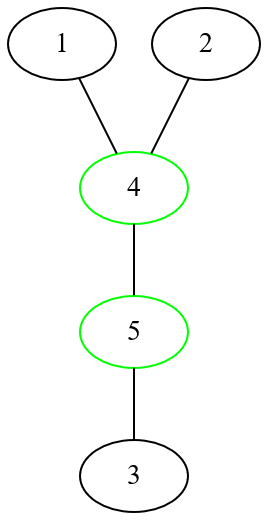
\includegraphics[width=0.2\textwidth]{sample-1.png}
  \end{figure}
\end{center}
The green spots are parts of the wood, and spots $1-3$ are houses. You can verify that the distances 
between each pair of houses matches those in the input.

\section*{Explanation of sample 2}
Given the distances of sample 2, Delsjön could look like what is shown below: 
\begin{center}
  \begin{figure}[h]
    \centering
    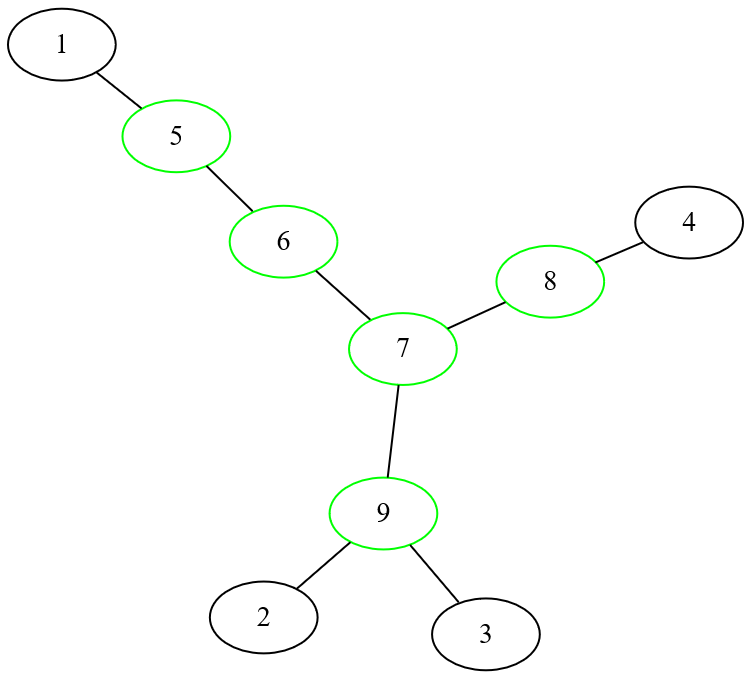
\includegraphics[width=0.4\textwidth]{sample-2.png}
  \end{figure}
\end{center}